\section{Architectural design}
\label{sect:overalldescription}

\subsection{Overview: High-level components and their interaction}
\label{subsect:Overview:Highlevelcomponentsandtheirinteraction}
\begin{figure}[h!]
    \centering
    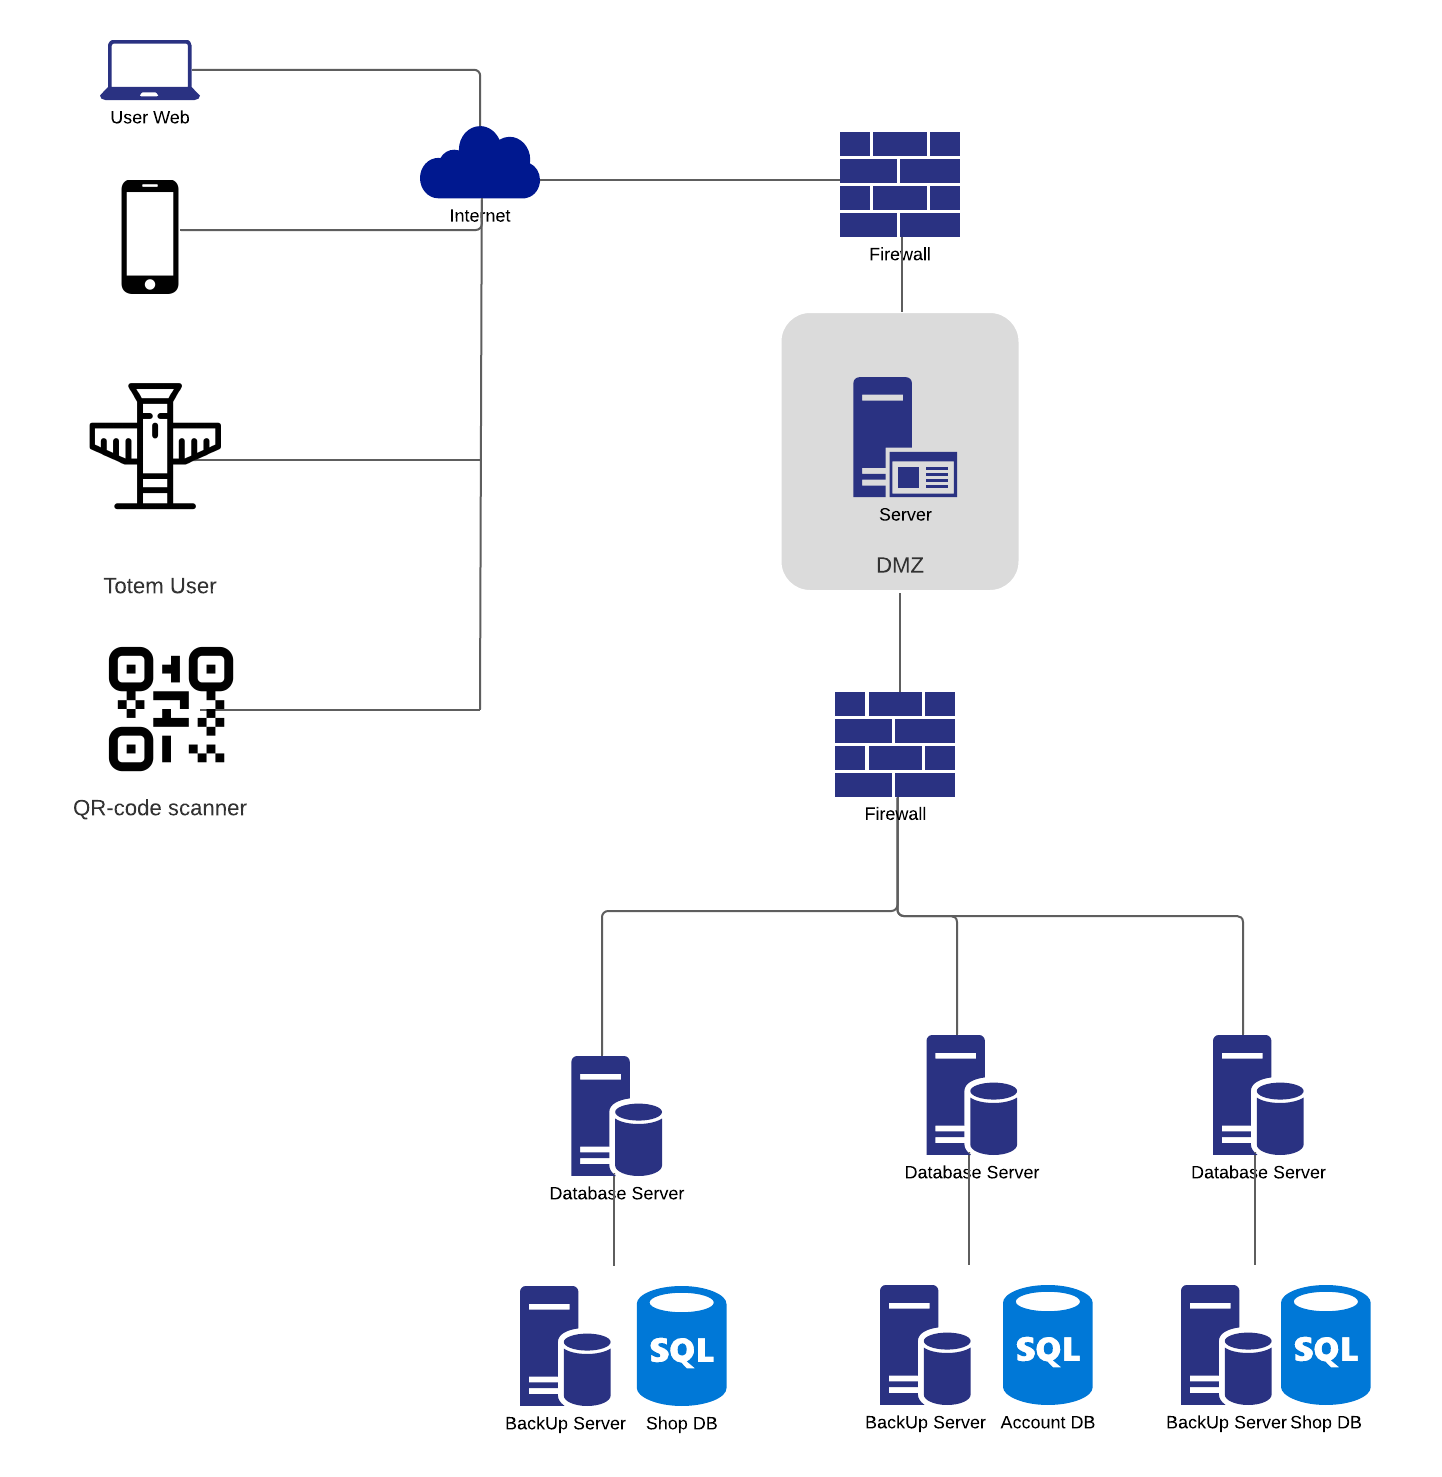
\includegraphics[width=0.6\textwidth]{Images/PhysicalDiagram.png}
    \caption{\label{fig:PhysicalDiagram}{Physical Diagram}}
\end{figure}
The architecture of the system can be divided into three logical layer: presentation layer, business layer and daya layer.\\
The presentation layer is the part of the application that manages the interface through which the user will actually experience and interact with our application. 
This layer will be managed either on the client side, for the offline functionalities and the static content, and on the server-side, for what concerns the dynamic content. 
It has been chosen to develop a cross-platform application: in order to do so, the front-end of the application will be developed according with the framework of React-Native.
Indeed, the front-end will be supported either by IOs and Android Devices, as well as Web browsers.
 In the figure, we see that our users can connect with the server-side of the application via mobile devices, laptop devices, Totem devices and the Qr-code Scanner.
Mobile devices will be trivially able to connect either via the native application or the browser-based application.
For what concerns the laptop users and the totem users, they will be able to connect to our application using only the browser-based application.
Qr-code scanner application, however, won't be implemented by us, who will just handle the HTTP requests incoming from it, so it won't be futrher discussed in this document.\\
The Business layer is the core of the application and connect the presentation layer and the data layer. It allow users to retrieve desired data and to have access to dedicated functionalities. We decided to implement our business layer using the Micro-Services architecture. This architecture divide the application in multiple tinier applications, each of which is mainly dedicated to a specific function. All of those improperly said functions coadiuvate in order to offer to the user the entire set of features offered by the application. This is the best way to implement an application which must be scalable, as CLup, which is a young start-up hoping to grow a lot. Furthermore, we decided to implement a cloud computing based application: through the joined use of Kubernetes and Docker it is possible to scale the resources needed dynamically and according to the incoming request, so that, with a IaaS approach, we will be able to reduce the costs to the essential.\\
By the way, each of our micro-services will need, in order to fulfill their duty, to store and retrieve several information. These information will be kept in dedicated SQL Data Bases through SQL DBMS, which represent the Data Layer. The data layer is the memory of our application and a significant part of it, so for each data base, a Back up database will be implmented either.\\


\subsection{Component view}
\label{subsect:componentview}
The following diagrams show the main components of the system and the interfaces through which they interact, the coloured, encircled ones are the one we are going to implement:
\begin{itemize}
    \item The client side is made of four components, which refer to the qr-code scanner application, to the web users and to the mobile application users.
    \item The server side is divided in three subsystems, each of them implements a specific service of the application. For the sake of clarity three different diagram has been modelled. The subsystems are:
    \begin{itemize}
        \item \textbf{Queue Services Subsystem}: it provides the interfaces needed either by managers and users in order to accesses to the functions correlated to the queue associated to a shop. A disambiguation is here needed, with the term "queue", here and in every other part of the document, we indicate a series of ticket in temporal order, either queue ticker or visit ticket.
        \item \textbf{Shop Services Subsystem}: it provides the interfaces needed by managers and users in order to accesses to the functions correlated to the shop.
        \item \textbf{Account Manager Services}: it provides the interfaces needed to manage the accounts and also implements security feature.
    \end{itemize}
\end{itemize}
\begin{figure}[h!]
    \centering
    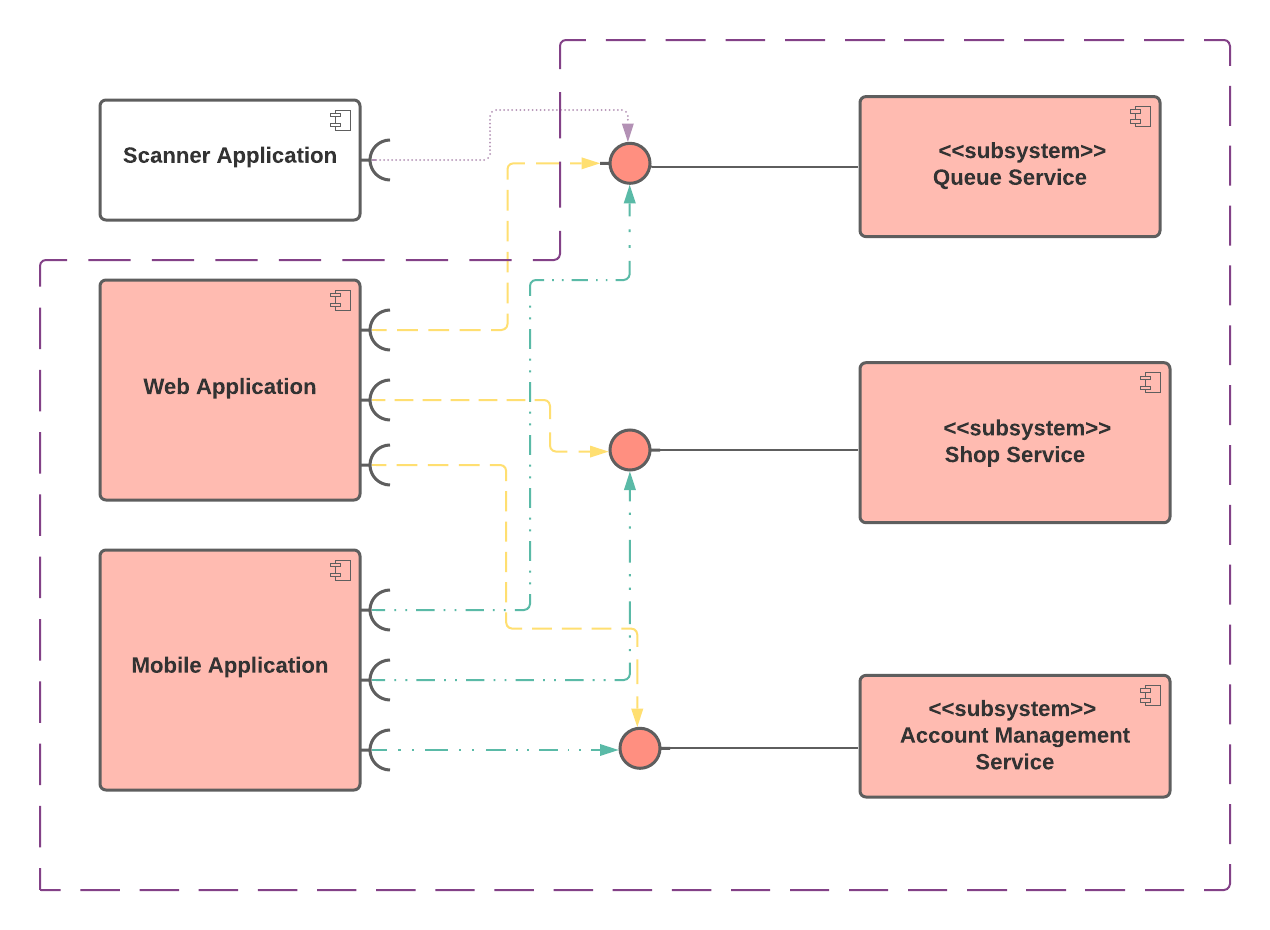
\includegraphics[width=0.6\textwidth]{Images/ComponentViewHighLevel (1).png}
    \caption{\label{fig:ComponentViewHighLevel}{General component view}}
\end{figure}

\textbf{Queue Service Subsystem Projection}
This service is divided into four components: \textit{Qr-code scanner component, Visit component, LineUp Component, Queue Info Component, Analytics Component, Ticket Generator Component, Notificate User Component and Data Manager Component}. 
The \textbf{Qr-code scanner Component} is a component dedicated to update the status of the ticket once they are scanned. It communicate with the QR-code scanner, offering it an interface through which it will be able to call it, in order to correctly fulfill its function.\\
The \textbf{Visit Component} is a component dedicated to the management of the visit tickets. It generate a ticket through the \textit{Ticket Generator Component} and decorate it as a visit ticket. It offers to the client a set of functionalities, such as book a visit or cancel a previous booked one.\\
The \textbf{LineUp Module} is a component dedicated to the management of the visit tickets. It generate a ticket through the \textit{Ticket Generator Component} and decorate it as a line ticket. It offers to the client a set of functionalities, such as the possibility to enqueue or to dequeue.\\
The \textbf{Queue Info Component} is a component dedicated to the retrievement of the information about the queue of a shop.
Indeed, it offers a dedicated interface to the clients. It may have the need to handle immediate information or analytical data. The latter, are calculated thanks to the \textit{Analytics Component}.\\
The \textbf{Analytics Component} is a component dedicated to the computation of analytical data about the queue.
The \textbf{Notificate User Component} is a component dedicated to the send push notification to the client. In order to so, it communicates with a Push Api.
Finally, the \textbf{Data Manager Component} is a component dedicated to interact with the Queue DBMS and offers an interface to all of the other component in the service in order to have access to it.

\begin{figure}[h!]
    \centering
    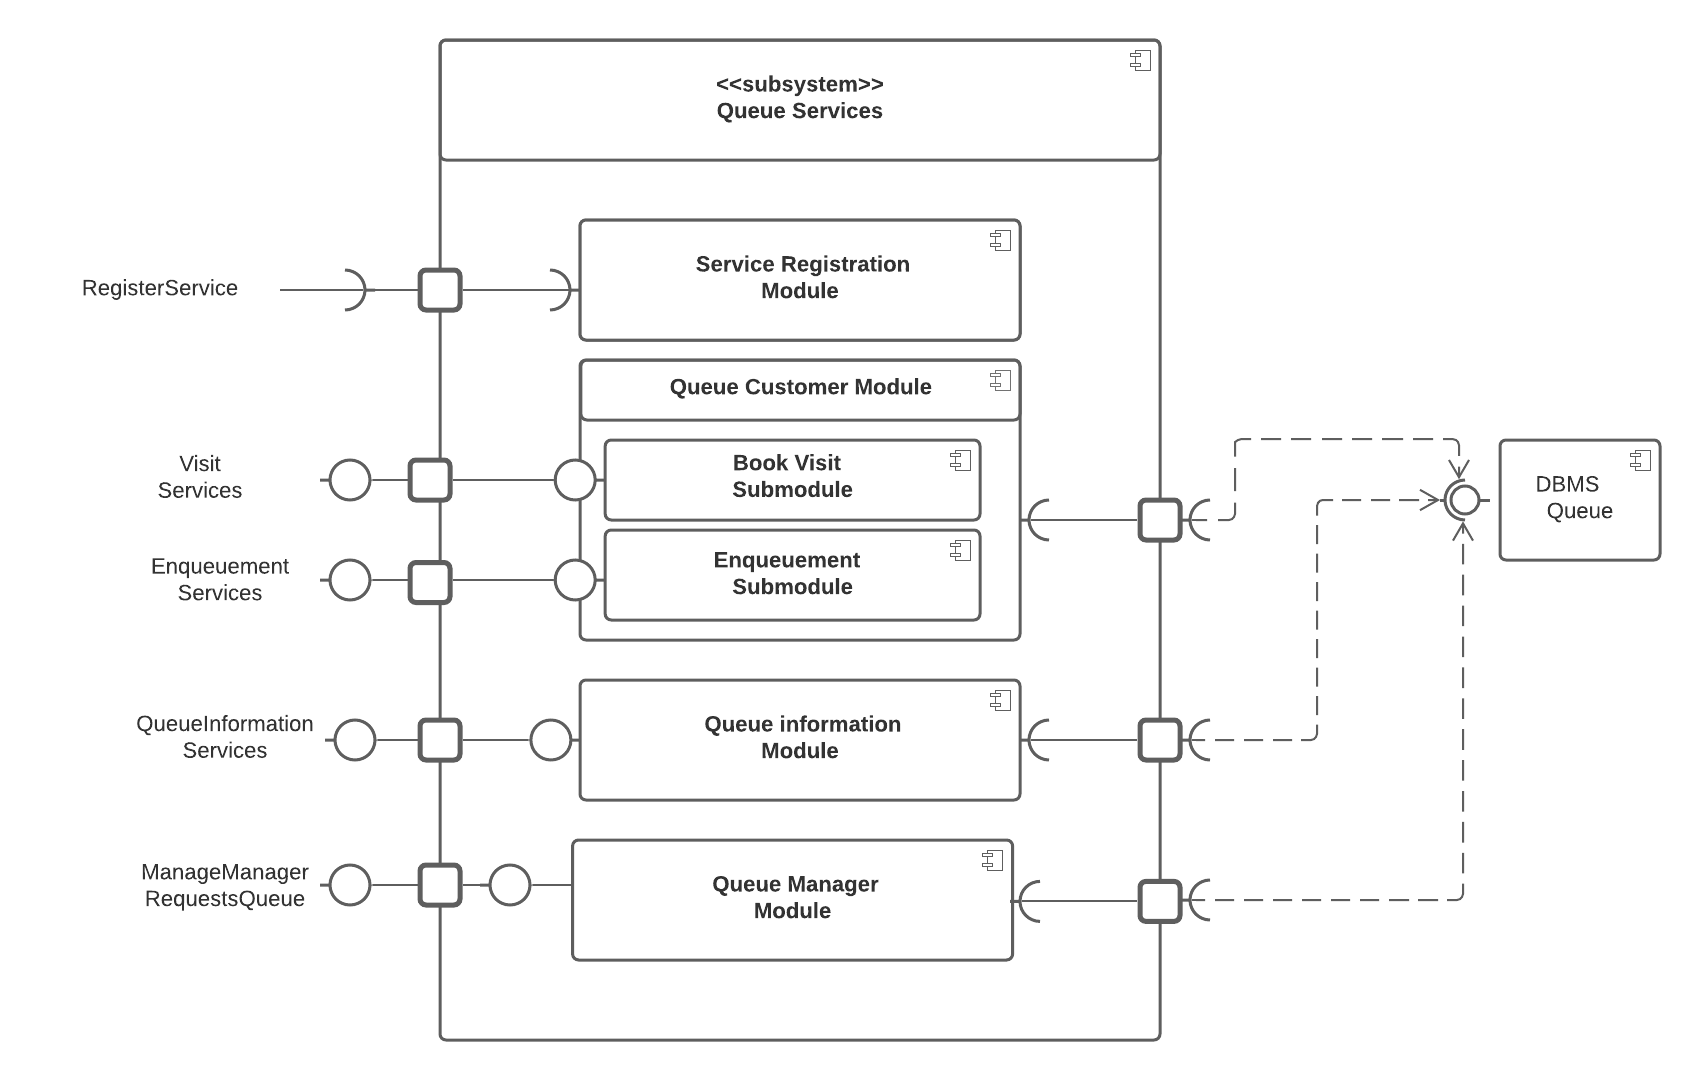
\includegraphics[width=0.6\textwidth]{Images/ComponentViewQueueService.png}
    \caption{\label{fig:ComponentViewQueueServices}{General component view}}
\end{figure}


\textbf{Shop Service Subsystem Projection}
This service is divided into three components: \textbf{Manage Shop Component, Shop Info Module, Data Manager Module}. \\
The \textbf{Manage Shop Component} is a component dedicated to features exploited by managers. It implements an interface which will allow a manager to add a shop and to update the information of a shop already registered in the system.
The \textbf{Shop Info Component} is a component which implements an interface that provides functions to retrieve information about a shop. This component, for some of its features, needs to communicate with the Maps Api.
Finally, the \textbf{Data Manager Component} is a component dedicated to interact with the Shop DBMS and offers an interface to all of the other component in the service in order to have access to it.

\begin{figure}[h!]
    \centering
    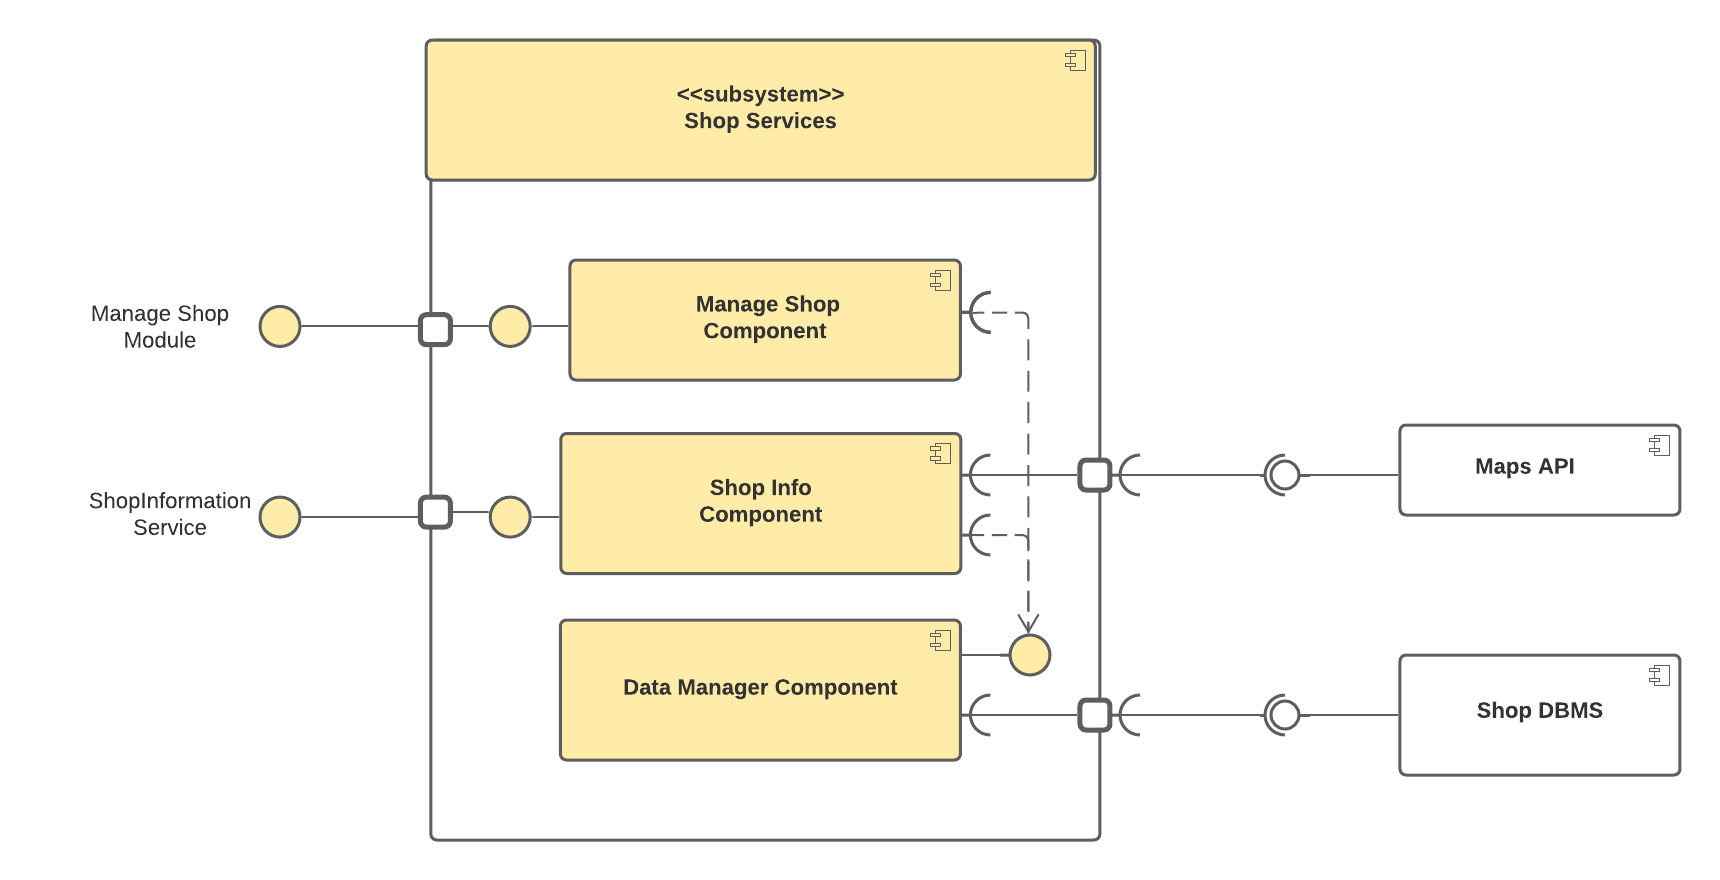
\includegraphics[width=0.6\textwidth]{Images/ComponentViewShopServices (1).png}
    \caption{\label{fig:ComponentViewShopServices}{General component view}}
\end{figure}

\textbf{Account Manager Subsystem Projection}
This service is divided into three components: \textbf{Account Manager Component, Authentication and Authorization Engine Component and the Data Manager Component}. \\
The \textbf{Account Manager Component} is a component dedicated to manage the clients accounts. It offer the clients an interface through which they can, for exempale, sign on, sign in or update their profile. It communicates with the\\
The \textbf{Authentication and Authorization Engine Component} which provides to it an interface with the functions needed in order identify and authenticate a user. It will need to communicate with the SMS gateway from time to time in order to accomplish its function.\\
The \textbf{Data Manager Component} is a component dedicated to interact with the Account DBMS and offers an interface to all of the other component in the service in order to have access to it. 

\begin{figure}[h!]
    \centering
    \caption{\label{fig:ComponentViewAccountManagerServices}{General component view}}
\end{figure}




\subsection{Entity-relationship diagram}
\label{subsect:entityrelationshipdiagram}

TODO:FEDE

\subsection{Deployment view}
\label{subsect:deploymentview}
The system architecture is a 4-Tier architecture, it is based on the JEE framework and it's typical of a Service Oriented Application:
\begin{itemize}
    \item \textbf{TIER 1} is the client tier, it is composed by the mobile applications, the totems and the users browsers and the qr-code scanner application. All of them will communicate with the web server via the HTTPS protocol.
    \item \textbf{TIER 2} is composed by the application server. This tier hosts the OS system CentOs, which will welcome the platform Kubernetes which, with the jointed effort of Docker, will orchestrate the ideal enviroment execution for our microservices application. Kubernetes, among its numerous services, offers an ELB api, through which will successfully dispatch correctly the incoming HTTP requests to the correct service. Each service will be deployed as a Docker Image directly by Kubernetes through a Docker File and will be hosted in a Docker container.
    \item \textbf{TIER 4} is the Data Tier. 
    We decided to implement 3 different Databases, one for each offered microservices. 
    The connection beetween Tier 2 and 3 is performed via JDBC connector which uses jdbc protocol.
\end{itemize}
\begin{figure}[h!]
    \centering
    \includegraphics[width=0.6\textwidth]{Images/Deployement View (2).png}
    \caption{\label{fig:Deployement View}{General component view}}
\end{figure}

copiata micidiale da power enjoy

\subsection{Runtime view}
\label{subsect:runtimeview}

\\TODO: cambia shop deployement view aggiungendo tickettometuser component


user search a shop

user book a visit/user enqueue (sono molto simili..)

customer line up (totem)

QR-code scanner

Manager cancels a customer visit

\subsection{Component interfaces}
\label{subsect:componentinterfaces}

Facciamo interfacce come power enjoy e specifichiamo che a ogni metodo corrisponde una servlet, e che il mezzo di comunicazione è HTTP, quindi non avremo effettivamente queste interfacce

\subsection{Selected architectural styles and patterns}
\label{subsect:selectedarchitecturalstylesandpatterns}

MVC

OBSERVER (per la view di sicuro, per il resto boh, dobbiamo capirlo)

CHAIN OF RESPONSIBILITY PATTERN – In this design pattern a request from a client can be handled by a number of handler or receiver objects. So basically, the client request is passed down each handler in the chain until a handler that can process the request is found. Servlet filters are a classic example of the Chain of Responsibility pattern. Spring has a class called HandlerInterceptorAdapter which is also an example of the Chain of Responsibility pattern. It has a method called preHandle, which follows the chain of responsibility pattern. Both servlet filters as well as Spring interceptors can be used to house code that is common for all requests like logging or authentication and that is separate from the business logic.

FACADE

SIGLETON - maybe

STRATEGY - maybe

POOL PATTERN - connection pooling patern JDBC - oppure no se usiamo JPA

TOMCAT GESTISCE LO SCHEDULING DEGLI EVENTI TEMPORALI..

\subsection{Other design decisions}
\label{subsect:otherdesigndecisions}


